\documentclass{beamer}

\usepackage[utf8x]{inputenc}
\usepackage{default}

\usepackage{amsmath}

\usepackage{multicol}
\usepackage{url}
\usepackage{graphicx}

%figures
%\usepackage{wrapfig}

%font
\usepackage[T1]{fontenc}
\usepackage{venturis}

\usecolortheme{beaver}

%titlepage
\title{Simulation of the unstable rotation of a cuboid}
\subtitle{Books in space}
\author{Ivar Postma \and Eamon Nerbonne}
\institute[University of Groningen]
{
  Introduction to Computational Science \\
  School for Computing and Cognition \\
  University of Groningen
}
\date{January 19, 2011}

\begin{document}

\frame{\titlepage}

\begin{frame}
 \frametitle{What you should remember from last time...}
 \begin{itemize}
  \item We looked at the rotation of a rigid body; a book
  \item We showed a clip of an experiment in space
  \item Rotation around two of the main axis is stable, rotation around the third is not
 \end{itemize}
\end{frame}

\begin{frame}
 \frametitle{String particle simulation}
 \begin{itemize}
  \item In the lecture on Molecular Dynamics we've seen how to simulate a vibrating string with particles
  \item Particles are connected by springs that create interacting forces
  \item From the forces we can calculate how to update the velocity of the points ($a = \frac{F}{m}$)
  \item From the velocity we can calculate how to update the position of points
 \end{itemize}
\end{frame}

\begin{frame}
 \frametitle{Particle simulation}
 \framesubtitle{Model of a book}
 \begin{itemize}
  \item We represent the book with 8 particles, located at the corners
  \item Each point has the same mass
  \item There is an interacting force (spring) between each pair of particles
  \item This force is proportional to the distance between the particles minus their initial distance
 \end{itemize}
 \pause
 \begin{figure}
  \centering
  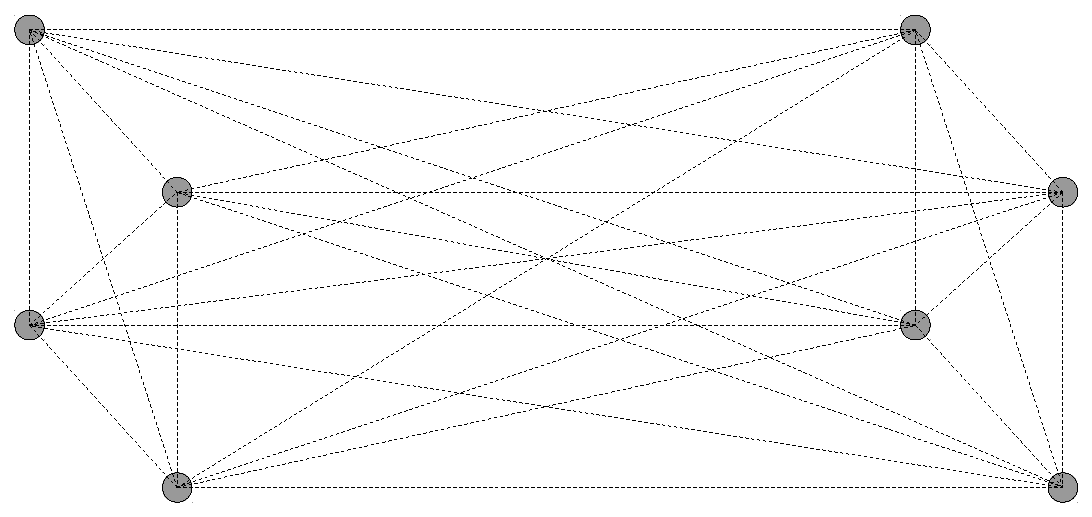
\includegraphics[width=0.7\textwidth]{strings.pdf}
 \end{figure}
\end{frame}

\begin{frame}
 \frametitle{Particle simulation}
 \framesubtitle{Computations}
 \begin{itemize}
  \item Calculate force on particle $i$:
  \begin{displaymath}
   F_i(t) = \sum_j (x_i(t) - x_j(t)) - (x_i(0) - x_j(0))
  \end{displaymath}
  \item Calculate velocity of particle $i$:
  \begin{displaymath}
   v_i(t) = v_i(t - \Delta t) + F_i(t) \times \Delta t
  \end{displaymath}
  \item Calculate position of particle $i$:
  \begin{displaymath}
   x_i(t) = x_i(t - \Delta t) + v_i(t) \times \Delta t
  \end{displaymath}
 \end{itemize}
\end{frame}

\begin{frame}
 \frametitle{Particle simulation}
 \framesubtitle{Computations}
 Using Euler integration, for $n$ particles, in each time step we need to compute
 \begin{itemize}
  \item $\frac{(n-1)^2}{2}$ forces
  \item $n$ velocities
  \item $n$ positions
 \end{itemize}
\end{frame}

\begin{frame}
 \frametitle{Particle simulation}
 \framesubtitle{Demonstration}
 \begin{figure}
  \centering
  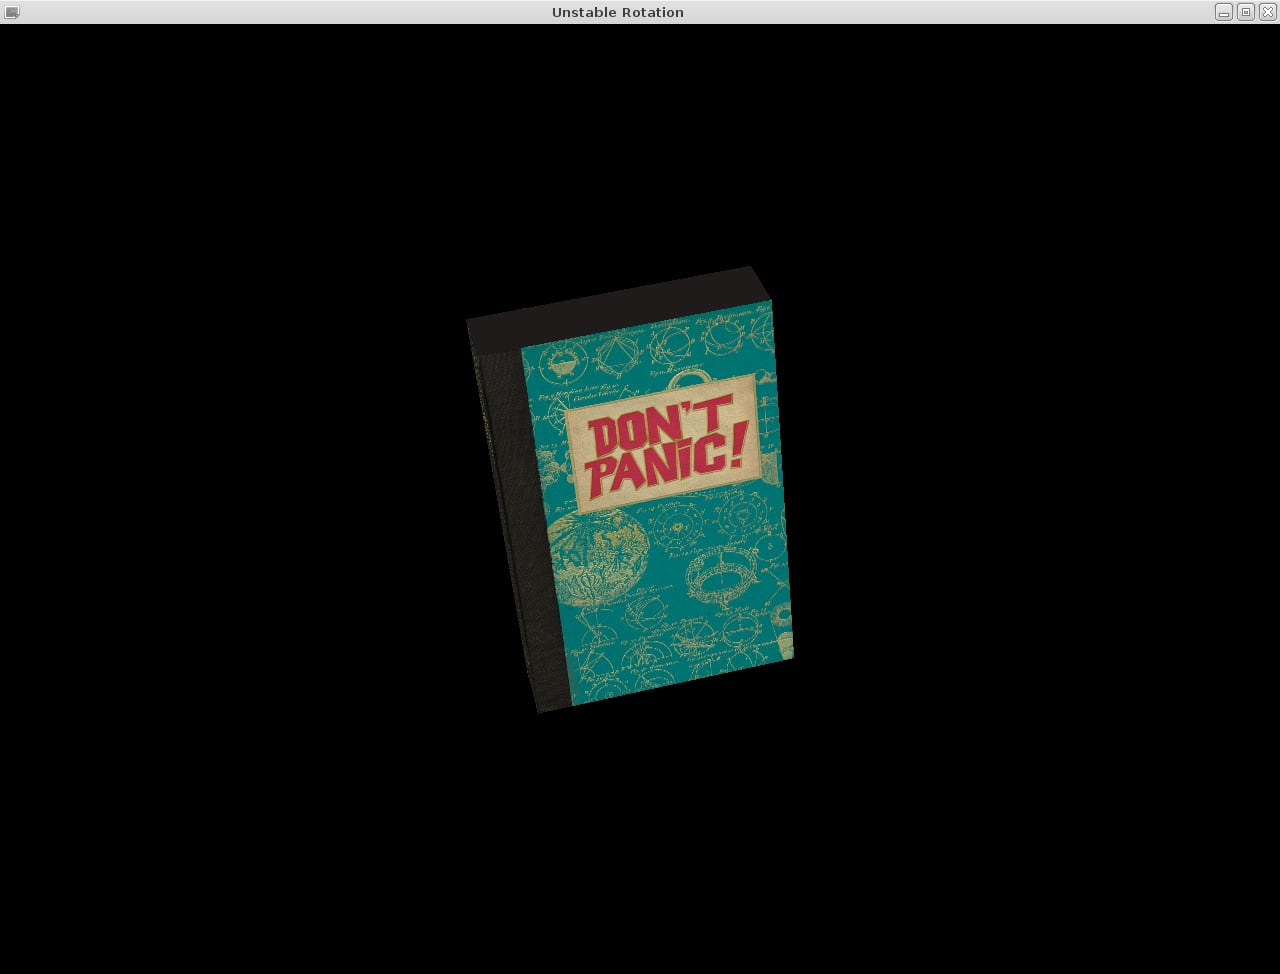
\includegraphics[width=0.7\textwidth]{demo.png}
 \end{figure}
\end{frame}

\begin{frame}
 \frametitle{Particle simulation}
 \framesubtitle{Observations}
 \begin{itemize}
  \item The book seems to behave naturally
  \item Rotation is stable around two axis and unstable around the third
  \item After some time the simulation ``explodes''
 \end{itemize}
\end{frame}

\begin{frame}
 \frametitle{Particle simulation}
 \framesubtitle{Normalisation}
 \begin{itemize}
  \item Euler integration introduces a small error in each time step
  \item Eventually, the shape of the book changes
  \item Other integration techniques can reduce the error, but not eliminate it
  \item We can normalise the model using the conservation of energy
 \end{itemize}
\end{frame}

\begin{frame}
 \frametitle{Particle simulation}
 \framesubtitle{Demonstration with normalisation}
 \begin{figure}
  \centering
  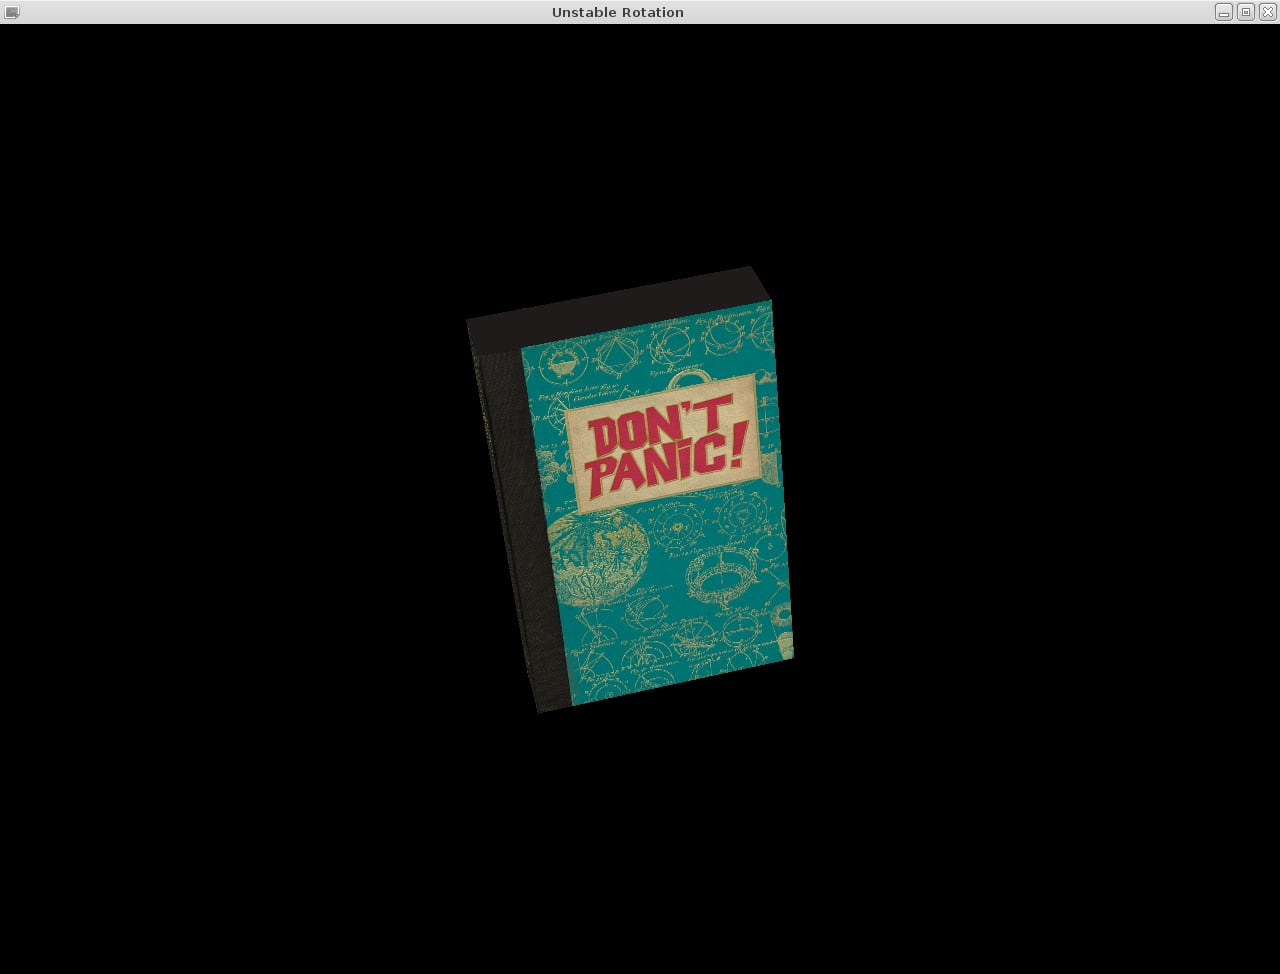
\includegraphics[width=0.7\textwidth]{demo.png}
 \end{figure}
\end{frame}

\begin{frame}
 \frametitle{Particle simulation}
 \framesubtitle{Normalisation}
 \begin{itemize}
  \item Energy is conserved
  \item Angular momentum is eventually transformed into vibration
 \end{itemize}
\end{frame}

\begin{frame}
 \frametitle{A different approach}
 \begin{itemize}
  \item In our previous presentation we mentioned a different approach
  \item In that model we calculate the angular velocity to update the orientation of the book
 \end{itemize}
\end{frame}

\begin{frame}
 \frametitle{Calculating the orientation}
 \begin{itemize}
  \item The angular velocity is calculated from the angular momentum and the moment of inertia
  \item The change in orientation is calculated from the angular velocity
 \end{itemize}

\begin{displaymath}
 I(t) = R(t - \Delta t) \times I_{body} \times R(t - \Delta t)^{T}
\end{displaymath}

\begin{displaymath}
 \omega(t) = I(t)^{-1} \times L
\end{displaymath}

\begin{displaymath}
 R(t) = R(t - \Delta t) + R(t - \Delta t) \times \omega^*(t) \times \Delta t
\end{displaymath}


\end{frame}

\begin{frame}
 \frametitle{Angular velocity based simulation}
 \framesubtitle{Demonstration}
 \begin{figure}
  \centering
  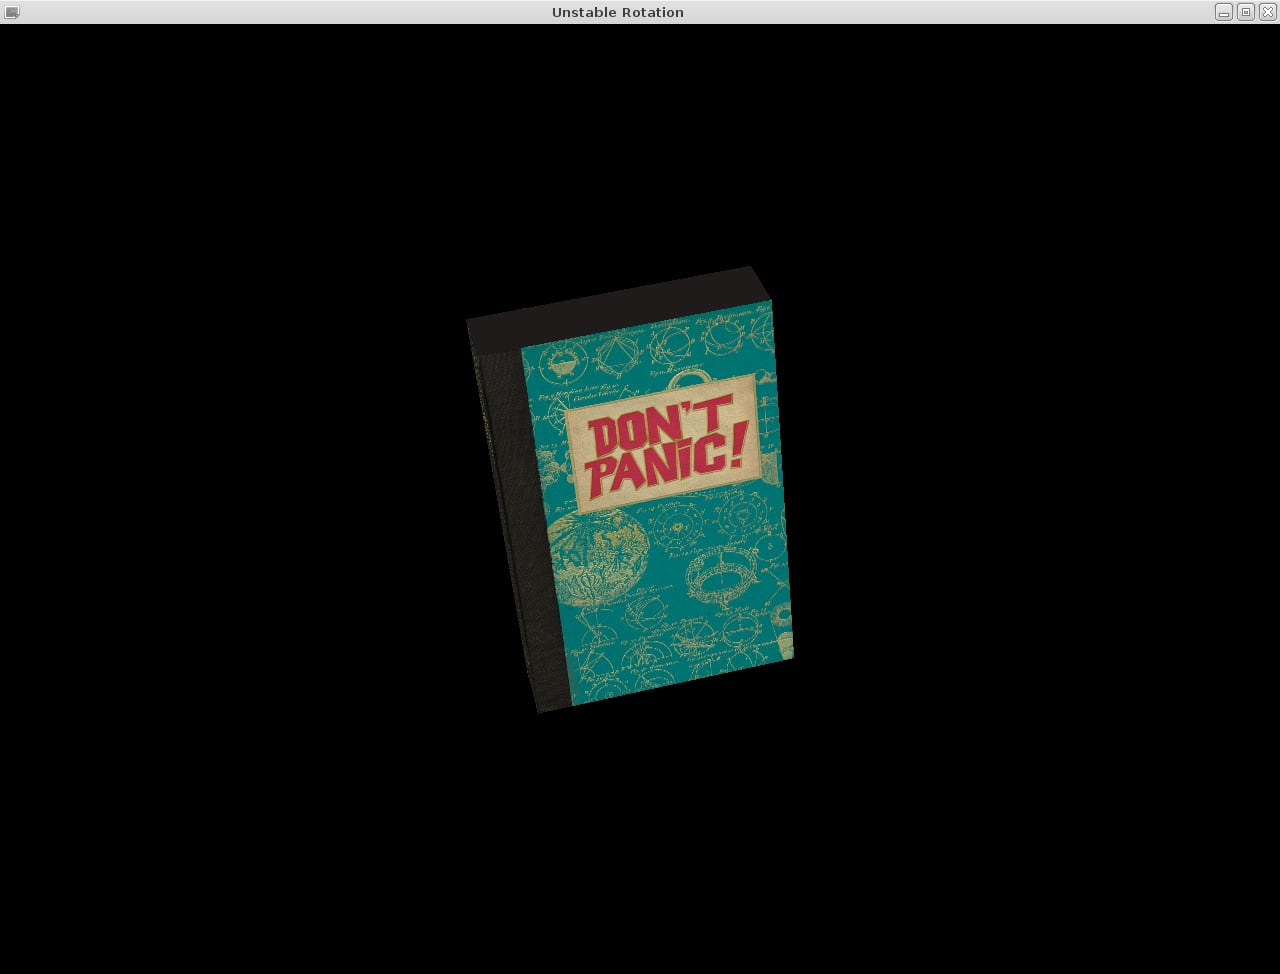
\includegraphics[width=0.7\textwidth]{demo.png}
 \end{figure}
\end{frame}

\begin{frame}
 \frametitle{Calculating the orientation} 
 \framesubtitle{Normalisation}
 \begin{itemize}
  \item Again, Euler integration introduces a small error in each time step
  \item Book changes shape
  \item The orientation can be normalised by singular value decomposition (SVD) of the matrix that describes the orientation
 \end{itemize}
\end{frame}

\begin{frame}
 \frametitle{Angular velocity based simulation}
 \framesubtitle{Demonstration with normalisation}
 \begin{figure}
  \centering
  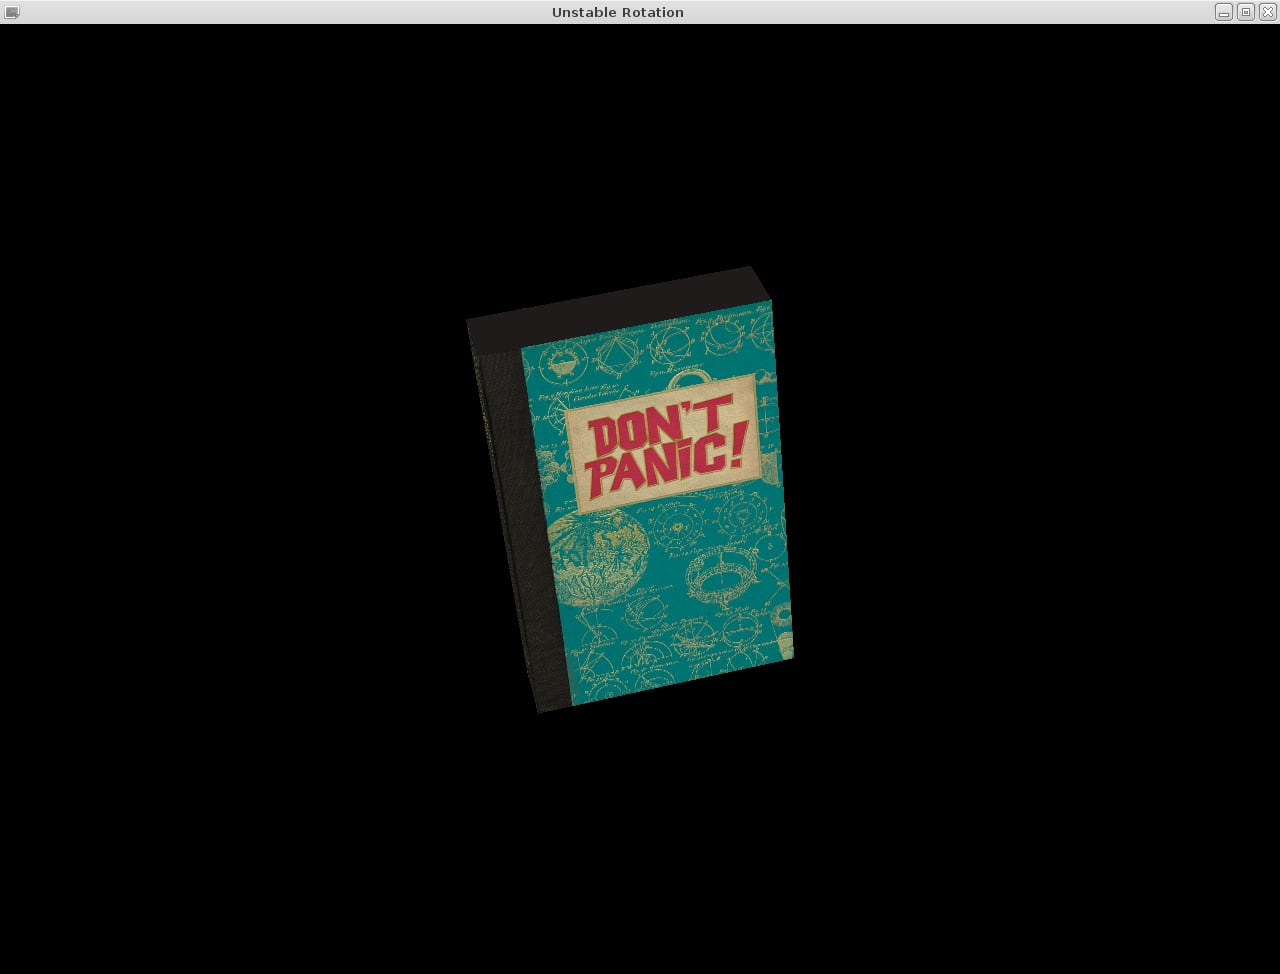
\includegraphics[width=0.7\textwidth]{demo.png}
 \end{figure}
\end{frame}

\begin{frame}
 \frametitle{Quaternions} 
 \begin{itemize}
  \item The orientation has 3 degrees of freedom, but in the model it's represented by a $3 \times 3$ matrix (9 degrees of freedom)
  \item Representing the orientation with quaternions reduces the degrees of freedom to 4
  \item Again, we want normalisation to prevent the shape from changing
 \end{itemize}
\end{frame}

\begin{frame}
 \frametitle{Angular velocity based simulation}
 \framesubtitle{Demonstration with quaternions}
 \begin{figure}
  \centering
  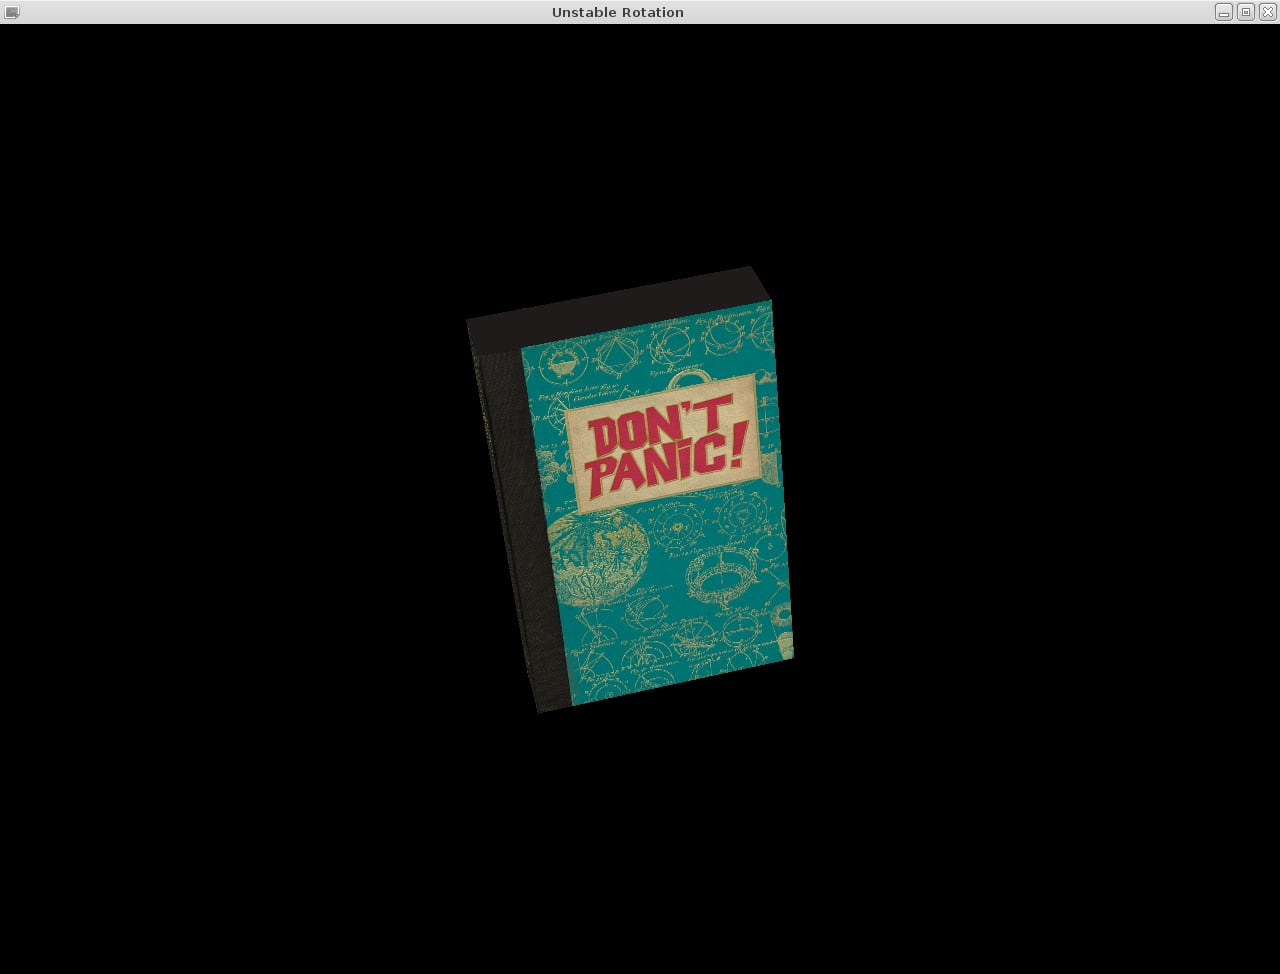
\includegraphics[width=0.7\textwidth]{demo.png}
 \end{figure}
\end{frame}

% \begin{frame}
%  \frametitle{Experiment in space}
%  \begin{figure}
%   \centering
%   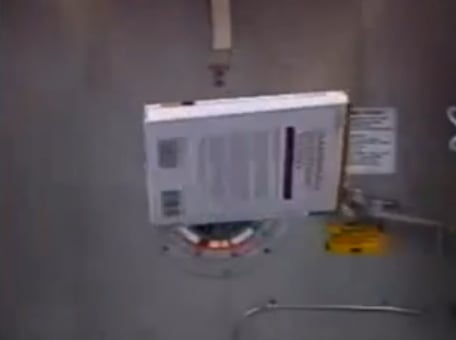
\includegraphics[width=0.4\textwidth]{book.png}
%  \end{figure}
% 
% 
%  \begin{itemize}
%   \item \url{http://www.youtube.com/watch?v=GgVpOorcKqc}
%  \end{itemize}
% \end{frame}
% 
% \begin{frame}
%  \frametitle{Stable and unstable rotation}
%  \begin{itemize}
%   \item The book can stably rotate around two of its axis
%   \item Rotation around the third axis is not stable
%  \end{itemize}
% \end{frame}
% 
% \begin{frame}
%  \frametitle{Model}
%  \framesubtitle{State}
%  A point is in a certain state
% 
%   \begin{table}
%   \centering
%     \begin{tabular}{ll}
%     $x(t)$ & position \\
%     $R(t)$ & orientation \\
%     $P(t)$ & total linear momentum \\
%     $L(t)$ & total angular momentum \\ 
%     \end{tabular}
%   \end{table}
% 
% \end{frame}
% 
% \begin{frame}
%  \frametitle{Model}
%  \framesubtitle{Updating the state}
%   \begin{table}
%   \centering
%     \begin{tabular}{ll}
%     $\dot{x}(t) = v(t)$ & velocity \\
%     $\dot{R}(t) = \omega^*(t) R(t)$ & angular velocity \\
%     $\dot{P}(t) = F(t)$ & force \\
%     $\dot{L}(t) = \tau(t)$ & torque (moment of force) \\ 
%     \end{tabular}
%   \end{table}
% 
% \begin{itemize}
%  \item $\omega^*(t)$ is the tensor notation of $\omega(t)$
%  \item $\dot{\alpha}$ is the notation for the time derivative of $\alpha$
% \end{itemize}
% 
% \end{frame}
% 
% \begin{frame}
%  \frametitle{Modelling the behaviour}
%  \framesubtitle{Simplifications}
%  We make a few simplifications
%  \begin{itemize}
%   \item The book is a cuboid
%   \item The density is uniform
%  \end{itemize}
% \end{frame}
% 
% \begin{frame}
%  \frametitle{Modelling the behaviour}
%  \framesubtitle{More simplifications}
%  When a book is rotating in space, the model is simple because
%  \begin{itemize}
%   \item there is no force, $F(t) = 0$
%   \item there is no torque, $\tau(t) = 0$
%   \item $x(t)$ is chosen to be the centre of mass, which is stationary
%  \end{itemize}
%  Thus, we only need to calculate the angular velocity
% \end{frame}
% 
% \begin{frame}
%  \frametitle{Model}
%  \framesubtitle{Updating the state}
% \begin{align*}
%     x & = \mbox{constant} \\
%     R(t + \epsilon) & = R(t) + \epsilon ~ \omega^*(t) R(t)\\
%     P & = 0 \\
%     L & = \mbox{constant}
% \end{align*}
% \end{frame}
% 
% \begin{frame}
%  \frametitle{Model}
%  \framesubtitle{Updating the state}
%  Angular speed is given by
%  \begin{displaymath}
%   \omega(t) = I(t)^{-1} L(t)
%  \end{displaymath}
% 
%  $I(t)$ depends on $R(t)$ and the moment of inertia of the body $I_{body}$
%  \begin{displaymath}
%   I(t) = R(t) I_{body} R(t)^{T}
%  \end{displaymath}
% \end{frame}
% 
% \begin{frame}
%  \frametitle{Moment of inertia}
%  \begin{itemize}
%   \item 
%   The moment of inertia of an object is a measure of the resistance of an object to changes in the rotation
% 
%   \item
%   For a cuboid the moment of inertia is given by
%   \begin{displaymath}
%     I_{body} = \frac{1}{12} \begin{pmatrix}
% 			    M(b^2 + c^2) & 0 & 0 \\
% 			    0 & M(a^2 + c^2) & 0 \\
% 			    0 & 0 & M(a^2 + b^2)
% 			    \end{pmatrix}
%   \end{displaymath}
%   where $a, b$ and $c$ are the dimensions of the cuboid
%  \end{itemize}
% \end{frame}
% 
% \begin{frame}
%  \frametitle{Methods to solve the calculations}
%  \begin{itemize}
%   \item Euler intergration
%   \item Midpoint method
%   \item 4th order Runga Kutta
%  \end{itemize}
% \end{frame}
% 
% \begin{frame}
%  \frametitle{Implementation}
%  We intend to implement this in C++ using OpenGL for the visualisation
% \end{frame}

\begin{frame}
 \frametitle{Conclusion}
 \begin{itemize}
  \item The (un)stable rotation of a book can be simulated with particles
  \item Eventually this simulation produces ``unnatural'' results
  \item In the other approach angular momentum is conserved
  \item This simulation is more robust
  \item But this only works when the moment of inertia of an object is known
 \end{itemize}
\end{frame}

 \begin{frame}
  \frametitle{Questions?}
 \end{frame}


\end{document}
